\documentclass[12pt,a4paper]{amsart}

\usepackage[croatian]{babel}
\usepackage[utf8]{inputenc}
\usepackage{amsmath,amssymb,amsfonts}
\usepackage{url}
\usepackage{mathtools}
\usepackage[dvipsnames,usenames]{color}
\usepackage{multirow}
\usepackage{tikz,lipsum,lmodern}
\usepackage[most]{tcolorbox}

% ne spreminjaj podatkov, ki vplivajo na obliko strani
\textwidth 15cm
\textheight 24cm
\oddsidemargin.5cm
\evensidemargin.5cm
\topmargin-5mm
\addtolength{\footskip}{10pt}
\pagestyle{plain}
\overfullrule=15pt % oznaci predlogo vrstico


% naslednje ukaze ustrezno popravi
\newcommand{\program}{Baze podataka} % ime studijskega programa: Matematika/Finan"cna matematika
\newcommand{\imeavtorja}{Lina Ivanova} % ime avtorja

\newcommand{\naslovdela}{Prva domaća zadaća}
\newcommand{\letnica}{2022} %letnica diplome

\begin{document}

% od tod do povzetka ne spreminjaj nicesar
\thispagestyle{empty}
\noindent{\large
PMF\\[1mm]
Matematički odsjek\\[5mm]
\program
\vfill

\begin{center}{\large
\imeavtorja\\[2mm]
{\bf \naslovdela}\\[10mm]
Baza podataka za Web Forum}
\end{center}
\vfill

\noindent{\large
Zagreb, \letnica}
\pagebreak

\thispagestyle{empty}
\tableofcontents
\pagebreak


\section{Introduction}
In the following document I will model and design a database for a forum - a web portal where ideas and views on a particular issue can be exchanged. \\
We want to model a database for a web forum on which different users can talk about a particular topic. Every user has an identification number for its account, which is created with email and password. The forum is constructed with sections which contain posts from specific topics. Hence every section has identification, name and only one moderator. The moderator is actually the user who made the particular section. Every user can start many discussions by making a post under particular section. Moreover every user can join a discussion with making a reply to the specific discussion. 

\section{Conceptual scheme}
The aforementioned database will be designed with the relational model. For that reason in the following part the problem will be graphically represented with the Chen diagram.

\subsection{Identifying the entities and relationships}
For the forum database we have identified the following entities and relationship:\\

\textbf{Entities:} User, section, discussion and reply.
\vspace{2mm}
\begin{itemize}
\item USER has the attributes identification number, email, username, password, registration date
\item SECTION has the attributes identification number, subject, number of posts
\item DISCUSSION has the attributes identification number, section, title, content
\item REPLY has the attributes identification number, content\\
\end{itemize}
The primary keys for our entities are: user identification number, section identification number, discussion identification number and reply identification number.\\

\textbf{Relationships:} Makes, posts, writes and belongs to.
\vspace{2mm}
\begin{itemize}
\item MAKES between USER and SECTION
\item POSTS between USER and DISCUSSION with an attribute date
\item WRITES between USER and REPLY with an attribute date
\item BELONGS TO between POST and SECTION\\
\end{itemize}
\vspace{4mm}
Next, for each relationship, we determine the \textbf{cardinality}:

\vspace{2mm}
\begin{itemize}
\item MAKES in direction from USER to SECTION has cardinality 0, M and in the opposite direction 1, 1
\item POSTS in direction from USER to DISCUSSION has cardinality 0, M and in the opposite direction 1, 1
\item WRITES in direction from USER to REPLY has cardinality 0, M and in the opposite direction 1, 1
\item IS UNDER in direction from DISCUSSION to SECTION has cardinality 0, M and in the opposite direction 1, 1\\
\end{itemize}

\subsection{Chen's diagram}
Once we have identified all the entities, relationships and attributes, we can now design the conceptual scheme of the database. For this purpose we will use a reduced Chen diagram. 

\begin{figure}[htbp]
\centerline{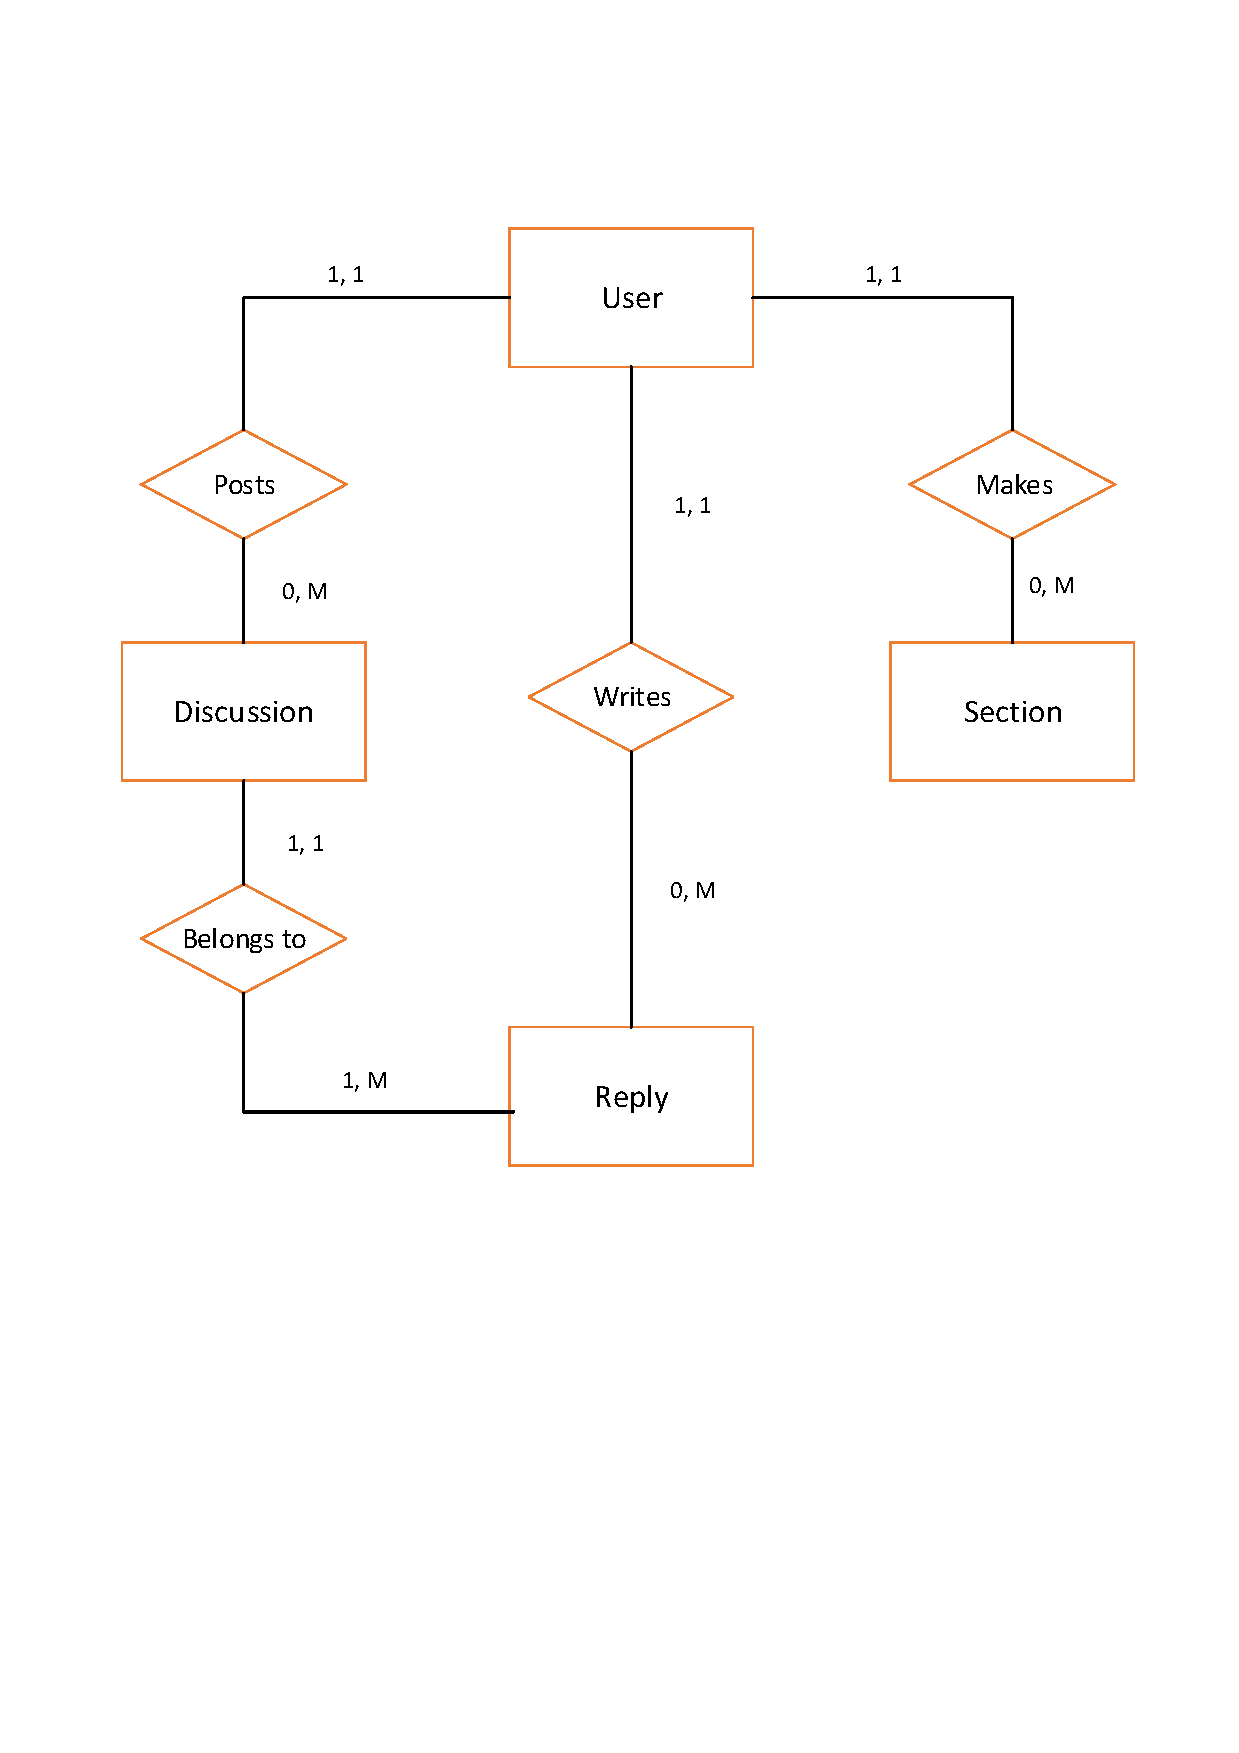
\includegraphics[scale=0.6]{Chen.pdf}}
\caption{Chen's diagram}
\label{fig1}
\end{figure}

\section{Relation scheme}
After the conceptual scheme was constructed we can move to the next step of the design process for database - the relation scheme. For our database of the Web Forum the scheme looks like this:\\
\vspace{2mm}

\begin{tcolorbox}[colback=orange!5!white,colframe=orange!75!black]
  USER(\underline{user\_id}, email, username, password, registration\_date)\\
  SECTION(\underline{section\_id}, user\_id, subject, no\_posts)\\
  DISCUSSION(\underline{discussion\_id}, user\_id, section\_id, title, discussion\_content, discussion\_date)\\
  REPLY(\underline{reply\_id}, user\_id, discussion\_id, reply\_content, reply\_date)\\
  POSTS(\underline{user\_id}, discussion\_id)
\end{tcolorbox}
\vspace{2mm}
The primary keys for our relations are respectively underlined in the above scheme. 

\section{Dictionary}
In the following section we will construct a dictionary for the data which will include all the attributes, their types and description of the entities. This can be shown in the next table.\\
\vspace{2mm}
\begin{center}
{\small 
\begin{tabular}{|c|c| p{7cm} |c|}
 \hline
 Name & Type & Decription \\
 \hline
 user\_id & integer & identification number that uniquely identifies every user \\ 
 \hline
 email & character & email addres of registered user \\ 
 \hline	
 username & character & username of user \\ 
 \hline
 password & character & password of user \\ 
 \hline
 registration\_date & timestamp & date when the user was registered \\ 
 \hline
 section\_id & integer & identification number that uniquely identifies every section \\ 
 \hline
 subject & character & name of the section \\ 
 \hline
 no\_posts & integer & number of discussion posted in the section \\ 
 \hline
 discussion\_id & integer & identification number that uniquely identifies every discussion \\ 
 \hline
 title & character & title of the discussion \\ 
 \hline
 discussion\_content & character & content of the discussion \\ 
 \hline
 section\_name & character & name of the section to which the discussion belongs \\ 
 \hline
 discussion\_date & timestamp & date of posting the discussion \\ 
 \hline
 reply\_id & integer & identification number that uniquely identifies every reply \\ 
 \hline
 reply\_content & character & content of the reply \\ 
 \hline
 reply\_date & timestamp & date of making the reply \\
 \hline
\end{tabular}
}
\end{center}

\end{figure}

%\item User(user_id, email, password, registration_date)
%\item Section(section_id, user_id, section_name, no_posts)
%\item Post(post_id, user_id, section_id, post_title, date, status)
%\item Reply(reply_id, user_id, date, time,



\end{document}
